\documentclass{scrreprt}

\usepackage{amsmath}
\usepackage{amsthm}
\usepackage{amssymb}
\usepackage{bm}
\usepackage[shortlabels]{enumitem}
\usepackage{hyperref}
\usepackage[utf8]{inputenc}
\usepackage{multicol}
\usepackage{mathtools}
\usepackage{pdflscape}
\usepackage{physics}
\usepackage{polynom}
\usepackage{tabularx}
\usepackage[table]{xcolor}
\usepackage{titling}
\usepackage{fancyhdr}
\usepackage{xfrac}
\usepackage{pgfplots}

\pgfplotsset{compat = newest}
\usepgfplotslibrary{fillbetween}
\usetikzlibrary{arrows, arrows.meta}
\usetikzlibrary{patterns}

% See https://tex.stackexchange.com/a/118217
\DeclarePairedDelimiter\ceil{\lceil}{\rceil}


\author{Karsten Lehmann}
\date{WiSe 2024/25}
\title{Übungsblatt 1\\INF-B-110, Diskrete Strukturen}

\setlength{\headheight}{26pt}
\pagestyle{fancy}
\fancyhf{}
\lhead{\thetitle}
\rhead{\theauthor}
\lfoot{\thedate}
\rfoot{Seite \thepage}

\begin{document}

\paragraph{Ü 1.1}
\begin{enumerate}[(a)]
\item Es werden Mengen {\color{red} $A \coloneqq \qty\big{
    x \in \mathbb{R} \:{\big|}\: -1 \leq x < 2
  }$} und {\color{blue} $B \coloneqq \qty\big{-2, -1} \cup \big(1,3\big]$}
  als Teilmenge der reellen Zahlen betrachtet.
  Bestimmen Sie die Mengen $A \cup B$, $A \cap B$ und $A \setminus B$.
  Skizzieren Sie $A \cross B$ in der euklidischen Ebene.

  \subparagraph{Lsg.}\:\\

    \begin{tikzpicture}[scale=2,>={Stealth[length=3mm]}]
      \draw[->] (-3,0) -- (4,0);
      \foreach \x in {-2, -1, 0, 1, 2, 3}
        \draw (\x, 0.1) -- (\x, -0.1) node[below] {\x};

      % Group A
      \draw[arrows={Bracket[]-Parenthesis[]}, very thick, red] (-1, 0.2) -- (2, 0.2);
      % Group B
      \draw[arrows={Parenthesis[]-Bracket[]}, very thick, blue] (1, 0.3) -- (3, 0.3);
      \node[circle, fill, inner sep=2pt, blue] at (-2, 0.3) {};
      \node[circle, fill, inner sep=2pt, blue] at (-1, 0.3) {};
    \end{tikzpicture}

  \begin{itemize}
  \item $A \cup B = \qty\big{-2} \cup \qty\big[-1, 3]$
  \item $A \cap B = \qty\big{-1} \cup \qty\big(1, 2)$
  \item $A \setminus B = \big(-1, 1\big]$
  \end{itemize}

    \begin{tikzpicture}[scale=2]
    \begin{axis}[
      axis x line=center,
      axis y line=center,
      grid=both,
      xmin=-2.1,
      xmax=3.1,
      xtick distance=1,
      ymin=-2.1,
      ymax=3.1,
      ytick distance=1,
    ]
      \draw[arrows={Bracket[]-Parenthesis[]}, very thick, blue] (-1, -1) -- (2, -1);
      \draw[arrows={Bracket[]-Parenthesis[]}, very thick, blue] (-1, -2) -- (2, -2);

      \draw[blue, name path=A, very thick] (-1, 1) -- (-1, 3) -- (2, 3);
      \draw[draw=none, name path=B] (2, 3) -- (2, 1);
      \addplot[pattern=north west lines, pattern color=blue] fill between [of=A and B];
    \end{axis}
  \end{tikzpicture}


\newpage
\item Es sei $S_i \coloneqq \qty\big{0, 1, \ldots, i}$ für alle
  $i \in \mathbb{N}$.
  Bestimmen Sie $\displaystyle \bigcup_{i \in \mathbb{N}} S_i$ und
  $\displaystyle \bigcap_{i \in \mathbb{N}} S_i$.

  \subparagraph{Lsg.} Es ist
  \[
    \bigcup_{i \in \mathbb{N}} S_i = \qty\big{
      n \in \mathbb{N} \:{\big |}\:
      \exists\; i \in \mathbb{N} \colon n \in S_i
    }
  \]
  Da für jedes $n \in \mathbb{N}$ gilt $n \in S_n$, folgt
  $\displaystyle \bigcup_{i \in \mathbb{N}} S_i = \mathbb{N}$.

  Außerdem ist 
  \[
    \bigcap_{i \in \mathbb{N}} S_i = \qty\big{
      n \in \mathbb{N} \:{\big |}\:
      \forall\; i \in \mathbb{N} \colon n \in S_i
    }
  \]
  Da für alle $n > 0$ die Menge $S_{n - 1}$ mit $n \notin S_{n - 1}$, folgt
  $\displaystyle \bigcap_{i \in \mathbb{N}} S_i = \qty\big{0}$

\item In der Vorlesung wurde bereits bewiesen, dass aus
  $\qty\big(a, b) = \qty\big(c, d)$ stets $a = c$ und $b = d$ folgt.
  Geben Sie ein Beispiel für Elemente $a$, $b$, $c$, $d$ an, so dass
  $\qty{a, \qty\big{b}} = \qty{c, \qty\big{d}}$ gilt, aber nicht
  $a = c$ und $b = d$.

  \subparagraph{Lsg.} Seien $b \neq d$ beliebig und
  $\underset{(1)}{\underbrace{a = \qty\big{d}}}$ sowie
  $\underset{(2)}{\underbrace{c = \qty\big{b}}}$.
  Dann ist
  \begin{flalign*}
    \qty\big{a, \qty\big{b}} &= \qty\big{\qty\big{d}, \qty\big{b}} &(1) && \\
                             &= \qty\big{\qty\big{d}, c} &(2) && \\
                             &= \qty\big{c, \qty\big{d}}
  \end{flalign*}
  Durch die Voraussetzung $b \ne d$, ist $\qty\big{b} \ne \qty\big{d}$ und
  $a \ne c$.

\item Bestimmen Sie für die Menge $A = \qty\big{\clubsuit, \heartsuit}$ die
  Potenzmenge $\mathcal{P}\qty\big(A)$.

  Wie groß ist die Mächtigkeit der Potenzmenge der Menge
  $B = \qty\big{\clubsuit, \heartsuit, \spadesuit, \diamondsuit}$

  \subparagraph{Lsg.} Es ist
  \[
    \mathcal{P}\qty\big(A) = \qty\Big{
      \emptyset, \qty\big{\clubsuit}, \qty\big{\heartsuit}, \qty\big{\clubsuit, \heartsuit}
    }
  \]

  Außerdem ist nach Kapitel 1.5 der Vorlesung
  $\abs{\mathcal{P}\qty\big(B)} = 2^{\abs{B}} = 2^4 = 16$.
\end{enumerate}

\newpage
\paragraph{Ü 1.2}
\begin{enumerate}[(a)]
\item Welche der folgenden Aussagen sind wahr, welche sind falsch?
  \begin{itemize}
  \item $\forall\: x \in \mathbb{Z} \:\exists\: y \in \mathbb{Z} \:\colon\: x = 2y$

    \subparagraph{Lsg.} Sei $x \in \mathbb{Z} = 3$.
    Dann ist $y = \frac{3}{2}$ als einzige Lösung für $x = 2y$ aus der Schulmathematik bekannt.
    Nun ist $y \notin \mathbb{Z}$.

    $\Rightarrow$ die Aussage ist \textbf{falsch}.

  \item $\forall\: x \in \mathbb{Z} \:\exists\: y \in \mathbb{Z} \:\colon\: x^2 + y^2 \geq 2xy$

    \subparagraph{Lsg.} Es ist
    \begin{flalign*}
      x^2 + y^2 &\geq 2xy & {\Big |}\: -2xy &&\\
      x^2 - 2xy + y^2 &\geq 0 \\
      (x - y)^2 &\geq 0
    \end{flalign*}
    und diese Ungleichung ist für alle $(x - y) \in \mathbb{Z}$ korrekt.

    $\Rightarrow$ die Aussage ist \textbf{wahr}.

  \item $\exists\: x \in \mathbb{Z} \:\forall\: y \in \mathbb{N} \:\colon\: x \leq y$

    \subparagraph{Lsg.} Sei $x \in \mathbb{Z} = 0$.
    Dann ist $0 \leq y \:\forall\: y \in \mathbb{N}$.

    $\Rightarrow$ die Aussage ist \textbf{wahr}.

  \item $\forall\: \epsilon \in \mathbb{R}, \epsilon > 0
    \:\exists\: n_0 \in \mathbb{N}
    \:\forall\: n \geq n_0 \:\colon\: \frac{1}{n} < \epsilon$

    \subparagraph{Lsg.} Sei $\epsilon \in \mathbb{R}, \epsilon > 0$ beliebig.
    Sei weiter $n_0 = \ceil{\frac{1}{\epsilon}} + 1$.
    Dann ist $n_0 \in \mathbb{N}$ und $\frac{1}{n_0} < \epsilon$ und
    $\frac{1}{n} \leq \frac{1}{n_0}$ für alle $n \geq n_0 \in \mathbb{N}$

    $\Rightarrow$ die Aussage ist \textbf{wahr}.
  \end{itemize}
\item Beschreiben Sie diejenigen $x \in \mathbb{Z}$, für die gilt:
  $\forall\: y \in \mathbb{Z}\:\exists\:z \in \mathbb{Z} \:\colon\:y = xz$

  \subparagraph{Lsg.} Es handelt sich um diejenigen $x$, für die gilt $x | y$.
\end{enumerate}

\newpage
\paragraph{Ü 1.3} Überprüfen Sie für jeder der folgenden Gleichungen, ob sie
für beliebige Teilmengen $A$, $B$ und $C$ einer Menge $M$ richtig oder falsch
sind.
Geben Sie einen Beweis bzw. ein Gegenbeispiel an.

\begin{enumerate}[(1)]
\item $A \cap \qty\big(B \setminus C) = \qty\big(A \cap B) \setminus C$

  \subparagraph{Lsg.} Es ist
  \begin{flalign*}
    A \cap \qty\big(B \setminus C)
    &= \qty\big{x \in A \:{\big |}\: x \in \qty\big{y \in B \:{\big |}\: y \notin C}} &\\
    &= \qty\big{x \in A \:{\big |}\: x \in B \text{ und } x \notin C} \\
    &= \qty\big{x \:{\big |}\: x \in A \text{ und }x \in B \text{ und } x \notin C} \\
    &= \qty\big{x \:{\big |}\: \qty\big(x \in A \text{ und }x \in B) \text{ und } x \notin C} \\
    &= \qty\big{x \:{\big |}\: x \in \qty\big(A \cap B) \text{ und } x \notin C} \\
    &= \qty\big(A \cap B) \setminus C
  \end{flalign*}

  $\Rightarrow$ \textbf{wahr}.

\item $\qty\big(A \cup B) \setminus B = \qty\big(A \setminus B) \cup B$

  \subparagraph{Lsg.} Seien $A = \qty\big{a}, B = \qty\big{b}$.
  Dann ist $\qty\big(A \cup B) \setminus B = \qty\big{a}$
  und $\qty\big(A \setminus B) \cup B = \qty\big{a, b}$.

  $\Rightarrow$ \textbf{falsch}.

\item $A \setminus \qty\big(A \setminus B) = A \cap B$

  \subparagraph{Lsg.} Es ist
  \begin{flalign*}
    A \setminus \qty\big(A \setminus B)
    &= \qty\big{x \in A \:{\big |}\: x \notin \qty\big{A \setminus B} } \\
    &= \qty\big{x \in A \:{\big |}\: x \notin \qty\big{y \in A \:{\big|}\: y \notin B} } \\
    &= \qty\big{x \in A \:{\big |}\: x \in \qty\big{y \notin A \:{\big|}\: y \in B} } & \text{Widerspruch zu $x \in A$} &&\\
    &= \qty\big{x \in A \:{\big |}\: x \in B } \\
    &= A \cap B
  \end{flalign*}

  $\Rightarrow$ \textbf{wahr}.
\end{enumerate}

\newpage
\begin{landscape}
  \paragraph{Ü 1.4}
  \begin{enumerate}[(a)]
  \item Wo befinden sich die sogenannten \emph{Dreieckszahlen}
    $\frac{\qty\big(n + 1)n}{2}$ im Pascalschen Dreieck?

    \subparagraph{Lsg.} Es ist
    \[
      \frac{\qty\big(n + 1)n}{2}
      = \frac{\qty\big(n + 1) \cdot n \cdot \qty\big(n - 1)!}{2! \qty\big(n - 1)!}
      = \frac{\qty\big(n + 1)!}{2! \qty\big(n + 1 - 2)!}
      = \binom{n + 1}{2}
    \]

    \begin{tabular}{>{$n=}l<{$\hspace{12pt}}*{13}{c}}
      0 &&&&&&&1&&&&&&\\
      1 &&&&&&1&&1&&&&&\\
      2 &&&&&$\binom{0 + 1}{2} = 1$&&2&&1&&&&\\
      3 &&&&1&&$\binom{1 + 1}{2} = 3$&&3&&1&&&\\
      4 &&&1&&4&&$\binom{2 + 1}{2} = 6$&&4&&1&&\\
      5 &&1&&5&&10&&$\binom{3 + 1}{2} = 10$&&5&&1&\\
      6 &1&&6&&15&&20&&$\binom{4 + 1}{2} = 15$&&6&&1
    \end{tabular}

  \item Bestimmen Sie alle $n \in \mathbb{N}, n \geq 3$, für die
    $\binom{n}{2} < \binom{n}{3}$ gilt.

    \subparagraph{Lsg.} Es ist
    \[
      \binom{n}{2} < \binom{n}{3}
      \iff \frac{n!}{2\qty\big(n - 2)!} < \frac{n!}{6\qty\big(n - 3)!}
      \iff \frac{n!}{2\qty\big(n - 2)\qty\big(n - 3)!} < \frac{n!}{6\qty\big(n - 3)!}
      \Rightarrow 2\qty\big(n - 2) > 6
      \Rightarrow n > 5
    \]

  \item In einer Menge von 17 Elementen befinden sich $A$ und $B$.
    Auf wie viele Arten kann man aus dieser Menge 12 Elemente entnehmen,
    dass die Regel \emph{``Falls man $A$ wählt, muss auch $B$ gewählt werden''}
    entnehmen?

    \subparagraph{Lsg.} Das ist Ziehen-ohne-Zurücklegen.
    Dabei sind relevant die Zahl der Möglichkeiten ohne $A$,
    $\binom{16}{12} = 1820$, die sowie die Zahl der Möglichkeiten 10 weiter
    Elemente zu ziehen, nachdem bereits sowohl $A$ als auch $B$ entnommen wurden,
    $\binom{15}{10} = 3003$.
    Also insgesamt $4823$.
  \end{enumerate}
\end{landscape}
\end{document}
